%% thesis.tex 2022/2/14
%
% Based on sample files of unknown authorship.
%
% The San Francisco State University LaTeX thesis template is
% derived from the UC Berkeley LaTeX thesis template. 
%
% The current maintainer of this work at San Francisco State University is Robert Browder.
%
% A healthy alternative to working directly in LaTeX is to use the thesisdown or bookdown package with R Studio.
% Thesis down provides the opportunity to embed executable code within the narrative flow of your document.
% Thesis down provides both PDF and HTML output.  
%
% This is the main file for this template
%
% This file is where authors may customize title, author, degree semester, degree year, degree, 
% chair, other members, and major.
%
% This file issues the commands to include each part of the document, 
% Pre-formatted parts available - abstract, preface, acknowledgments, introduction, chap1, chap2, 
% and references
% Any part can be omitted by commenting out its "include" command
% Authors may also rearrange the order of contents and add additional chapters using the mark-up examples provided


\documentclass{sfsuthesis}
\usepackage{biblatex}

% Use the graphix package with dvipdfmx when exporting to HTML to preserve figure dimensions for JPG and PNG file types. 
% For this to work you must first create an .xbb file for each file using the following command from the CLI
% ebb -x Picture2.jpg
% \usepackage[dvipdfmx]{graphicx}

% Use the graphix package without dvipdfmx when exporting to PDF
\usepackage{graphicx}
\usepackage{amsmath}
\usepackage{rotating} % provides sidewaystable and sidewaysfigure

% To compile this file from the command line, run "latex thesis", then "biber thesis"
% (or "bibtex thesis", if the output from latex asks for that instead),
% and then "latex thesis" (without the quotes in each case).
%
% Alternatively, use Overleaf, MacTeX, or MikTeX to compile to PDF.
%
% To compile this file to HTML from the command line, run 
%  make4ht -f html5+mjcli thesis.tex "mathjax"
% this step requires Nodes.js, MathJax, and mjcli.js to be installed and working on your machine


% comment out the following two lines for single spacing
\def\dsp{\def\baselinestretch{2.0}\large\normalsize}
\dsp

% comment out the following line to control indentation of the first paragraph of a section
\usepackage{indentfirst}
\usepackage{appendix}

\addtolength{\abovecaptionskip}{\baselineskip}

\newtheorem{theorem}{Sample Text}

\bibliography{references}

\hyphenation{mar-gin-al-ia}
\hyphenation{bra-va-do}

%path to the folder which contains figures
\graphicspath{ {./figures/} }

\begin{document}

% Declarations for Front Matter

\title{Formal Verification of Neural Networks using Semi-Definite Programming}
\author{Michael Andrew Roark}
\degreesemester{Fall}
% Select one of the semesters: December, May, or August.
\degreeyear{2022}
% Enter the year in which you are submitting your thesis.
\degree{Masters of Arts}
%example: Masters of Science
\chair{Serkan Hosten}
\chairdegree{Ph.D}
\chairrank{Professor}

\cochair{Henry Baoteng}
\cochairdegree{Ph.D}
\cochairrank{Associate Professor}

\memberthree{Tao He}
\memberthreedegree{Ph.D}
\memberthreerank{Associate Professor}

\memberfour{Name of Member Four}
\memberfourdegree{Ph.D}
\memberfourrank{Associate Professor}
\othermembers{Professor Roger Spam \\
  Associate Professor Michael Chex}
% For a co-chair who is subordinate to the \chair listed above
% \cochair{Professor Benedict Francis Pope}
% For two co-chairs of equal standing (do not use \chair with this one)
% \cochairs{Professor Richard Francis Sony}{Professor Benedict Francis Pope}
\numberofmembers{3}

\field{Mathematics}
% Example: Computer Science: Software Engineering
% Designated Emphasis -- this is optional, and rare
% \emphasis{Colloidal Telemetry}
% This is optional, and rare
% \jointinstitution{University of Western Maryland}
% This is optional (default is Berkeley)
% \campus{Berkeley}


\maketitle
% Delete (or comment out) the \approvalpage line for the final version.
\copyrightpage
\approvalpage


% (This file is included by thesis.tex; you do not latex it by itself.)
\begin{abstract}

% The text of the abstract goes here.  If you need to use a \section
% command you will need to use \section*, \subsection*, etc. so that
% you don't get any numbering.  You probably won't be using any of
% these commands in the abstract anyway.

Begin your abstract here.

\end{abstract}


\begin{frontmatter}

\begin{preface}

Including a Preface for your work is optional. If you do not have one, please delete this page.
\end{preface}

% You can delete the \clearpage lines if you don't want these to start on
% separate pages.


\begin{acknowledgments}
Normally the Acknowledgments section gives you the opportunity to thank those to whom you are indebted for assistance in the project. This should be done briefly and in good taste.

\end{acknowledgments}

\tableofcontents
\clearpage
\listoftables
\clearpage
\listoffigures
\clearpage

\end{frontmatter}

% (This file is included by thesis.tex; you do not latex it by itself.)

\begin{introduction}

% If you need to use a \section
% command you will need to use \section*, \subsection*, etc. so that
% you don't get any numbering.  You probably won't be using any of
% these commands in the abstract anyway.

Lorem ipsum dolor sit amet, consectetuer adipiscing elit. Maecenas porttitor congue massa. Fusce posuere, magna sed pulvinar ultricies, purus lectus malesuada libero, sit amet commodo magna eros quis urna. Nunc viverra imperdiet enim. Fusce est. Vivamus a tellus.
Pellentesque habitant morbi tristique senectus et netus et malesuada fames ac turpis egestas. Proin pharetra nonummy pede. Mauris et orci. Aenean nec lorem. In porttitor. Donec laoreet nonummy augue.\par

Suspendisse dui purus, scelerisque at, vulputate vitae, pretium mattis, nunc. Mauris eget neque at sem venenatis eleifend. Ut nonummy. Fusce aliquet pede non pede. Suspendisse dapibus lorem pellentesque magna. Integer nulla.\par

\section*{Method}
Donec blandit feugiat ligula. Donec hendrerit, felis et imperdiet euismod, purus ipsum pretium metus, in lacinia nulla nisl eget sapien. Donec ut est in lectus consequat consequat. Etiam eget dui. Aliquam erat volutpat. Sed at lorem in nunc porta tristique.
Proin nec augue. Quisque aliquam tempor magna. Pellentesque habitant morbi tristique senectus et netus et malesuada fames ac turpis egestas. Nunc ac magna. Maecenas odio dolor, vulputate vel, auctor ac, accumsan id, felis. Pellentesque cursus sagittis felis.


\end{introduction}


\pagestyle{headings}

% (Optional) \part{First Part}

\chapter{Add a Chapter Title Here if you Wish}



Pellentesque porttitor, velit lacinia egestas auctor, diam eros tempus arcu, nec vulputate augue magna vel risus. Cras non magna vel ante adipiscing rhoncus. Vivamus a mi. Morbi neque. Aliquam erat volutpat. Integer ultrices lobortis eros. Rosa Olin Jackson\cite{waveshaping} ad litora torquent per conubia nostra.\par

Pellentesque habitant morbi tristique senectus et netus et malesuada fames ac turpis egestas. Proin semper, ante vitae sollicitudin posuere, metus quam iaculis nibh, vitae scelerisque nunc massa eget pede. Sed velit urna, interdum vel, ultricies vel, faucibus at, quam. Donec elit est, consectetuer eget, consequat quis, tempus quis, wisi. In in nunc. Class aptent taciti sociosqu ad litora torquent per conubia nostra, per inceptos hymenaeos.\par

\begin{figure}
\caption{Example of a basic figure title}
%Use the scale parameter to size the image
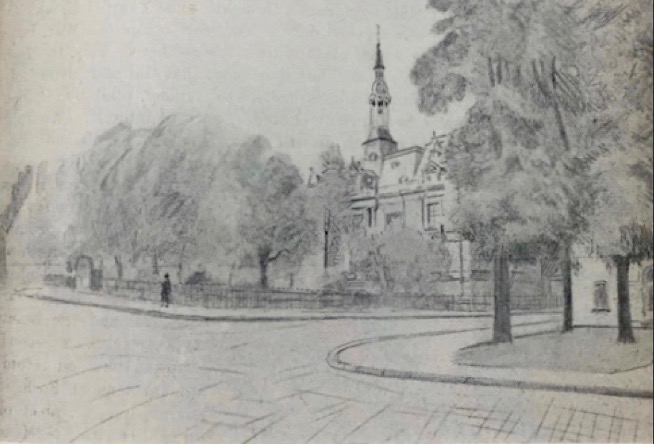
\includegraphics[width=1\textwidth]{Picture1}

% here is an alternate way to scale images based on specific sizes
%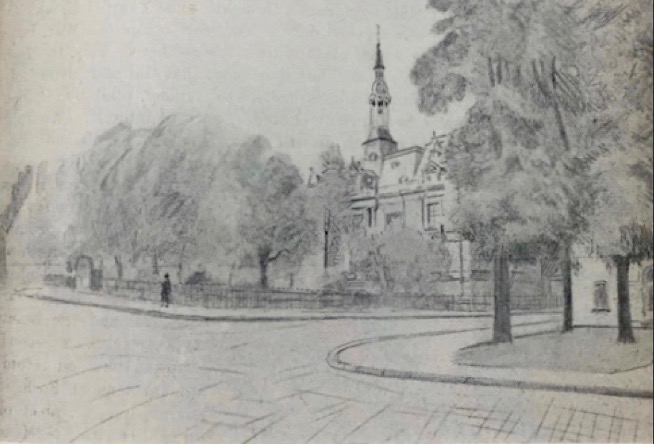
\includegraphics[width=5cm, height=4cm]{Picture1}
 \emph{This is an example of an image caption or description}
\end{figure}

Donec ullamcorper fringilla eros. Fusce in sapien eu purus dapibus commodo. Cum sociis natoque penatibus et magnis dis parturient montes, nascetur ridiculus mus.\par

% To remove the numeric value of the subheading below, insert an asterisk after \section (i.e., \section*)

\section{Chapter 1 Heading 3 (subheading)}

Cras faucibus condimentum odio. Sed ac ligula. Aliquam at eros. Etiam at ligula et tellus ullamcorper ultrices. In fermentum, lorem non cursus porttitor, diam urna accumsan lacus, sed interdum wisi nibh nec nisl. Ut tincidunt volutpat urna. Mauris eleifend nulla eget mauris. Sed cursus quam id felis. Curabitur posuere quam vel nibh. Cras dapibus dapibus nisl.\par

Vestibulum quis dolor a felis congue vehicula. Maecenas pede purus, tristique ac, tempus eget, egestas quis, mauris. Curabitur non eros. Nullam hendrerit bibendum justo. Fusce iaculis, est quis lacinia pretium, pede metus molestie lacus, at gravida wisi ante at libero. Quisque ornare placerat risus. Ut molestie magna at mi. Integer aliquet mauris et nibh. Ut mattis ligula posuere velit. Nunc sagittis.\par

\subsection{\emph{Chapter 1 Heading 4 (Sub-heading)}}

Curabitur varius fringilla nisl. Duis pretium mi euismod erat. Maecenas id augue. Nam vulputate. Duis a quam non neque lobortis malesuada. Praesent euismod. Donec nulla augue, venenatis scelerisque, dapibus a, consequat at, leo. Pellentesque libero lectus, tristique ac, consectetuer sit amet, imperdiet ut, justo. Sed aliquam odio vitae tortor. Proin hendrerit tempus arcu. In hac habitasse platea dictumst. Suspendisse potenti.\par
\chapter{}

\section{Sub-heading}

Vivamus vitae massa adipiscing est lacinia sodales. Donec metus massa, mollis vel, tempus placerat, vestibulum condimentum, ligula. Nunc lacus metus, posuere eget, lacinia eu, varius quis, libero. Aliquam nonummy adipiscing augue. Lorem ipsum dolor sit amet, consectetuer adipiscing elit. Maecenas porttitor congue massa. Fusce posuere, magna sed pulvinar ultricies, purus lectus malesuada libero, sit amet commodo magna eros quis urna. Nunc viverra imperdiet enim.

% This is an example of a simple table
\begin{table}
\centering
\begin{tabular}{|c|c|c|}
\hline
1-2-3 & yes & no \\
\hline
Multiplan & yes & yes \\
\hline
Wordstar & no & no \\
\hline
\end{tabular}
\caption{This is an example of a simple table.}
\end{table}

Fusce est. Vivamus a tellus. Pellentesque habitant morbi tristique senectus et netus et malesuada fames ac turpis egestas. Proin pharetra nonummy pede. Mauris et orci. Aenean nec lorem. In porttitor.\par

Donec laoreet nonummy augue. Suspendisse dui purus, scelerisque at, vulputate vitae, pretium mattis, nunc. Mauris eget neque at sem venenatis eleifend. Ut nonummy. Fusce aliquet pede non pede. Suspendisse dapibus lorem pellentesque magna. Integer nulla. Donec blandit feugiat ligula.\par


% This is an example of a more complex table
\begin{table}
\centering
\begin{tabular}{|ccccc|}
\hline
\textbf{Mitre} & \textbf{Enchantress} & \textbf{Hagstrom} &
\textbf{Atlantica} & \textbf{Martinez} \\
\hline
Arabic & Spicebush & Sapient & Chaos & Conquer \\
Jail & Syndic & Prevent & Ballerina & Canker \\
Discovery & Fame & Prognosticate & Corroborate & Bartend \\
Marquis & Regal & Accusation & Dichotomy & Soprano \\
Indestructible  & Porterhouse & Sofia & Cavalier & Trance \\
Leavenworth & Hidden & Benedictine & Vivacious & Utensil \\
\hline
\end{tabular}
\caption{This is an example of a slightly more complex table}
\end{table}

Donec hendrerit, felis et imperdiet euismod, purus ipsum pretium metus, in lacinia nulla nisl eget sapien. Donec ut est in lectus consequat consequat. Etiam eget dui. Aliquam erat volutpat. Sed at lorem in nunc porta tristique. Proin nec augue. Quisque aliquam tempor magna. Pellentesque habitant morbi tristique senectus et netus et malesuada fames ac turpis egestas.\par

\begin{figure}
\caption{Example of a basic figure title}
%Use the scale parameter to size the image
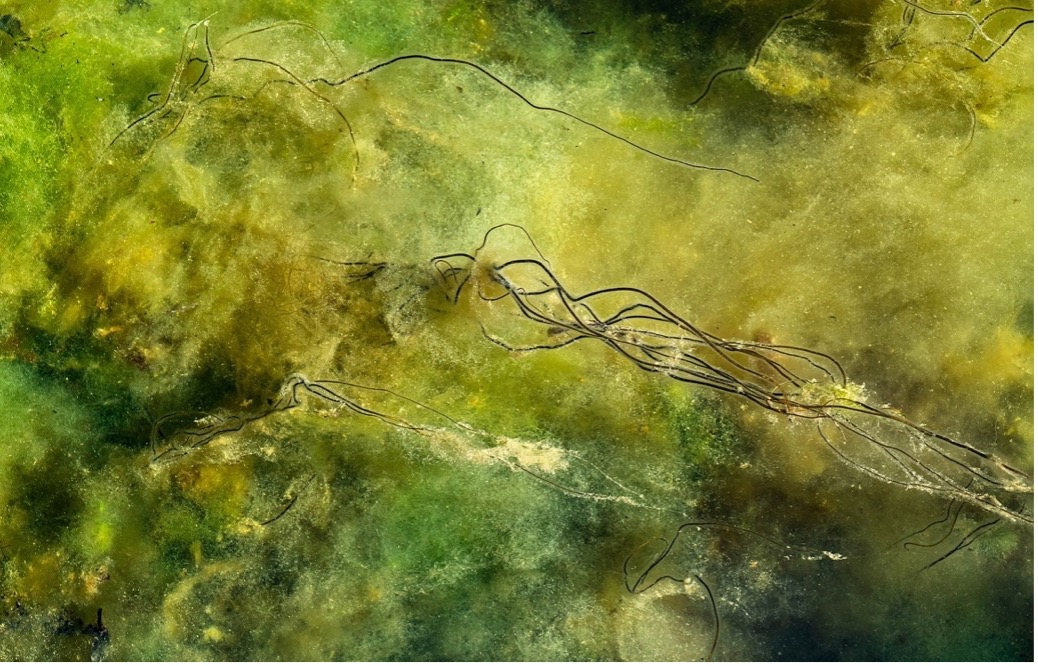
\includegraphics[scale=.45]{Picture2}

% here is an alternate way to scale images based on specific sizes
%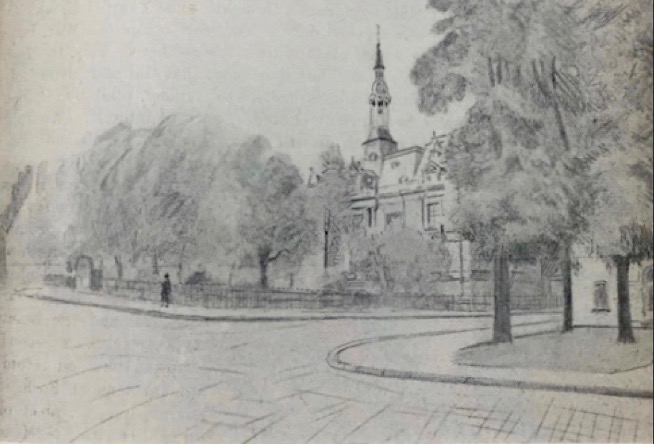
\includegraphics[width=5cm, height=4cm]{Picture1}
 \emph{This is an example of an image caption or description}
\end{figure}

Nunc ac magna. Maecenas odio dolor, vulputate vel, auctor ac, accumsan id, felis. Pellentesque cursus sagittis felis. Pellentesque porttitor, velit lacinia egestas auctor, diam eros tempus arcu, nec vulputate augue magna vel risus. Cras non magna vel ante adipiscing rhoncus. Vivamus a mi. Morbi neque. Aliquam erat volutpat. Integer ultrices lobortis eros. Pellentesque habitant morbi tristique senectus et netus et malesuada fames ac turpis egestas.\par

Proin semper, ante vitae sollicitudin posuere, metus quam iaculis nibh, vitae scelerisque nunc massa eget pede. Sed velit urna, interdum vel, ultricies vel, faucibus at, quam. Donec elit est, consectetuer eget, consequat quis, tempus quis, wisi. In in nunc. Class aptent taciti sociosqu ad litora torquent per conubia nostra, per inceptos hymenaeos. Donec ullamcorper fringilla eros. Fusce in sapien eu purus dapibus commodo.\par


% This is an example of figure drawn using code
\begin{figure}\centering
\parbox{.4\textwidth}{\centering
\begin{picture}(70,70)
\put(0,50){\framebox(20,20){}}
\put(10,60){\circle*{7}}
\put(50,50){\framebox(20,20){}}
\put(60,60){\circle*{7}}
\put(20,10){\line(1,0){30}}
\put(20,10){\line(-1,1){10}}
\put(50,10){\line(1,1){10}}
\end{picture}
\caption{Donec eu condimentum.}}
\hfill
\parbox{.4\textwidth}{\centering
\begin{picture}(70,70)
\put(0,50){\framebox(20,20){}}
\put(10,60){\circle*{7}}
\put(50,50){\framebox(20,20){}}
\put(60,60){\circle*{7}}
\put(20,10){\line(1,0){30}}
\put(20,10){\line(-1,-1){10}}
\put(50,10){\line(1,-1){10}}
\end{picture}
\caption{Quisque dapibus dignissim.}}
\end{figure}

Nam ac viverra dolor, sed pulvinar justo. Nullam orci est, ultrices non justo vel, euismod aliquet ligula. Cras semper, purus sed pharetra rhoncus, metus mauris ultricies odio, non sodales odio est finibus velit.

% Block quote example
\begin{quote}
This is an example of a block quote. Donec id mi at nulla tempor tincidunt a sit amet mi. Vivamus pulvinar dolor felis. Mauris in tellus accumsan, pellentesque lacus eu, aliquet lectus. Suspendisse felis nulla, scelerisque at maximus ut, mollis laoreet nisi. Pellentesque pulvinar libero pharetra dolor blandit pulvinar. Proin dapibus sodales velit ac rhoncus.
\end{quote}

Donec id mi at nulla tempor tincidunt a sit amet mi. Vivamus pulvinar dolor felis. Mauris in tellus accumsan, pellentesque lacus eu, aliquet lectus. Suspendisse felis nulla, scelerisque at maximus ut, mollis laoreet nisi. Pellentesque pulvinar libero pharetra dolor blandit pulvinar. Proin dapibus sodales velit ac rhoncus. Integer lacinia justo et enim porta porta. Praesent odio velit, ultrices interdum tortor in, consectetur bibendum dolor.

% This is an example of how to use footnotes
This is an example of a footnote.\footnote{This is the text that will appear in the footnote} Pellentesque libero lectus, tristique ac, consectetuer sit amet, imperdiet ut, justo. Sed aliquam odio vitae tortor. Proin hendrerit tempus arcu. In hac habitasse platea dictumst. Suspendisse potenti.


\begin{theorem}
\tolerance=10000\hbadness=10000
This is an example of how to use the theorem environment.
\end{theorem}


% Here as another example of a figure that has been drawn progammatically
\begin{figure}
\parbox{1\textwidth}{\centering
\begin{picture}(90,50)
  \put(0,0){\circle*{5}}
  \put(0,0){\vector(1,1){31.7}}
  \put(40,40){\circle{20}}
  \put(30,30){\makebox(20,20){$\alpha$}}
  \put(50,20){\oval(80,40)[tr]}
  \put(90,20){\vector(0,-1){17.5}}
  \put(90,0){\circle*{5}}
\end{picture}
\caption{ Here we see an example of a figure which has been drawn programatically using \LaTeX}}
\end{figure}

\begin{sidewaystable}
\centering
\begin{tabular}{|ccccc|}
\hline
\textbf{Mitre} & \textbf{Enchantress} & \textbf{Hagstrom} &
\textbf{Atlantica} & \textbf{Martinez} \\
\hline
Arabic & Spicebush & Sapient & Chaos & Conquer \\
Jail & Syndic & Prevent & Ballerina & Canker \\
Discovery & Fame & Prognosticate & Corroborate & Bartend \\
Marquis & Regal & Accusation & Dichotomy & Soprano \\
Indestructible  & Porterhouse & Sofia & Cavalier & Trance \\
Leavenworth & Hidden & Benedictine & Vivacious & Utensil \\
\hline
\end{tabular}
\caption{Here we have an example of a table that has been set in landscape}
\end{sidewaystable}


\begin{itemize}
\item This is an example of a bulleted list.
\item Praesent vestibulum mi turpis, vitae ultricies diam porttitor non.
\item Morbi sed vulputate nibh, ac iaculis odio.
\item Mauris ac risus eget eros ornare.
\item Proin quis tellus non velit posuere pulvinar.
\item Vestibulum tincidunt tempor hendrerit.
\item Praesent ornare imperdiet diam, sit amet laoreet.
\end{itemize}


\begin{enumerate}
\item This is an example of a numbered list.
\item Praesent vestibulum mi turpis, vitae ultricies diam porttitor non.
\item Morbi sed vulputate nibh, ac iaculis odio.
\item Mauris ac risus eget eros ornare.
\item Proin quis tellus non velit posuere pulvinar.
\item Vestibulum tincidunt tempor hendrerit.
\item Praesent ornare imperdiet diam, sit amet laoreet.
\end{enumerate}

\section{Math Examples}

Here we see an equation placed within an equation environment\par

\section{Math Examples}

Here we see an equation placed within an equation environment\par
\begin{equation}
cos (2\theta) = {\cos^2}\theta - \sin^2 \theta
\end{equation}

Here we see an equation which has not been placed in an equation environment\par
$
\lim\limits_{x \to \infty} \exp(-x) = 0
$

Here we have several more math examples\par
$
k_{n+1} = n^2 + k_n^2 - k_{n-1}
$

$
f(n) = n^5 + 4n^2 + 2 |_{n=17}
$

$
\frac{n!}{k!(n-k)!} = {n}{k}
$

$\frac{\frac{1}{x}+\frac{1}{y}}{y-z}$

\begin{equation}
\frac{
    \begin{array}[b]{r}
      \left( x_1 x_2 \right)\\
      \times \left( x'_1 x'_2 \right)
    \end{array}
  }{
    \left( y_1y_2y_3y_4 \right)
  }
\end{equation}

$\sqrt{\frac{a}{b}}$

$\sqrt[n]{1+x+x^2+x^3+\dots+x^n}$

$\sum_{i=1}^{10} t_i$

$\displaystyle\sum_{i=1}^{10} t_i$

$P\left(A=2\middle|\frac{A^2}{B}>4\right)$








\printbibliography

\appendix
\addappheadtotoc



\section{Appendix A: List of California State University Campuses}

\begin{itemize}
\item California State University, Bakersfield
\item California State University Channel Islands
\item California State University, Chico
\item California State University, Dominguez Hills
\item California State University, East Bay
\item California State University, Fresno
\item California State University, Fullerton
\item Humboldt State University
\item California State University, Long Beach
\item California State University, Los Angeles
\item California State University Maritime Academy
\item California State University, Monterey Bay
\item California State University, Northridge
\item California State Polytechnic University, Pomona
\item California State University, Sacramento
\item California State University, San Bernardino
\item San Diego State University
\item San Francisco State University
\item San José State University
\item California Polytechnic State University, San Luis Obispo
\item California State University San Marcos
\item Sonoma State University
\item California State University, Stanislaus
\end{itemize}


\section{Appendix B: Abbreviations of California State University Campuses}

\begin{itemize}
\item CSU Bakersfield
\item CSU Channel Islands
\item Chico State
\item CSU Dominguez Hills
\item Cal State East Bay
\item Fresno State
\item Cal State Fullerton
\item Humboldt State
\item Cal State Long Beach
\item Cal State LA
\item Cal Maritime
\item CSU Monterey Bay
\item CSUN
\item Cal Poly Pomona
\item Sacramento State
\item Cal State San Bernardino
\item San Diego State
\item San Francisco State
\item San José State
\item Cal Poly San Luis Obispo
\item CSU San Marcos
\item Sonoma State
\item Stanislaus State
\end{itemize}

\begin{subappendices}
\subsection{Sub Appendix}
\end{subappendices}



\end{document}
